\chapter{Design and Implementation}
\label{chapterlabel4}

The analysis performed in Chapter \ref{chapterlabel3} allows a full outline of the system requirements, the entities of the system and their assigned interactions, and leads onto the development of the full design of the software. The design phase starts with the design and the architecture of the system that is going to be built.




\section{Architecture and System Structure}
\label{Architecture_And_System_Structure}

The system is a typical B/S (Browser/Server) framework with a client browser sending requests and responses and a Kestrel server which is the default cross-platform HTTP server for ASP.NET Core projects. The server is running c\# (version 7.0) with a MySQL database. The server implementation listens for HTTP requests and surfaces them to the app as sets of request features composed into an HttpContext \cite{aspNetStructure}. ASP.NET Core communicates with the MySQL database which is hosted in Azure. The structure of ASP.NET Core is shown in figure \ref{asp_structure}.



\begin{figure}[h]
\begin{center}
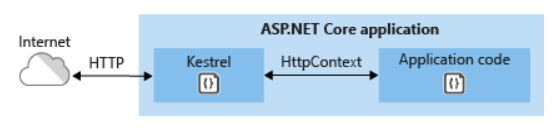
\includegraphics[width=17cm]{imgs/asp_structure.jpg}
\end{center}\vspace{-0.3cm}
\caption[ASP.NET Structure]{ASP.NET Structure} \label{asp_structure}
\end{figure}


The architectural framework is divided into four basic tiers: front-end, back-end, database, and file storage.

\begin{enumerate}
\item \textbf{Front-End}: the front end is user interface where the user completes a series of operations to control the application which is supported by HTTP request and HTTP response. It contains HTML code, JavaScript, JQuery and CSS)

\item \textbf{Back-End} when a static HTTP response is received from the web browser, ASP.NET Core will create an HttpRequest object that contains the request data, and invoke the correspondent view to handle this object. After the handle process, it will create and return a new HttpResponse object to the front-end view.
\item \textbf{Database}: ASP.NET Core controls the MySQL relational database which is hosted in Azure.
\item \textbf{File Storage}: The files selected by the user are uploaded to Azure Blob Storage.


\end{enumerate}

\begin{figure}[h]
\begin{center}
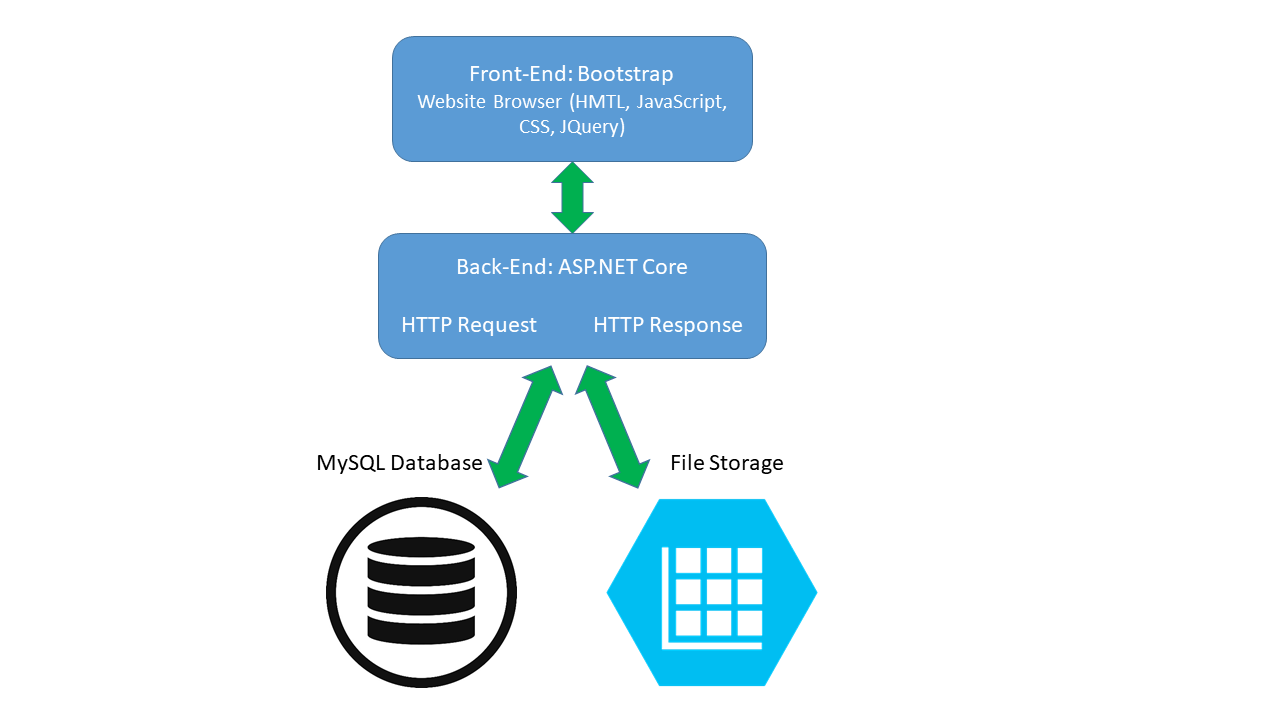
\includegraphics[width=17cm]{imgs/Application_Structure.png}
\end{center}\vspace{-0.3cm}
\caption[Application General Structure]{Application General Structure} \label{app_Structure}
\end{figure}


\section{Model-View-Controller Pattern}
\label{sub:MVC}

Due to the time limitations of the project the lack of experience in web designing, it was more appropriate to create a basic user interface and the devote the majority of the time to developing a robust back-end. Therefore, it was very important that the architecture of the application made a separation between the user interface and the back-end processing.

MVC framework is a one of the most popular design patterns which is motivated by the separation of the  UI and the processing performed to generate it. The MVC has been conceptualised for many years, and thus it precedes the inception of web applications and therefore, many efforts at applying the model to web applications through frameworks have been controversial.

Since most of the time has been devoted into developing the back-end than the front-end of the application, it is quite likely that at some point in the future the front-end would be replaced with a more aesthetically pleasing one.


The Model-View-Controller (MVC) architectural pattern separates an application into three main groups of components: Models, Views, and Controllers. This pattern helps to achieve separation of concerns \cite{separationOfConcerns}. Using this pattern, user requests are routed to a Controller which is responsible for working with the Model to perform user actions and/or retrieve results of queries. The Controller chooses the View to display to the user, and provides it with any Model data it requires \cite{mvc}. 

\begin{figure}[h]
\begin{center}
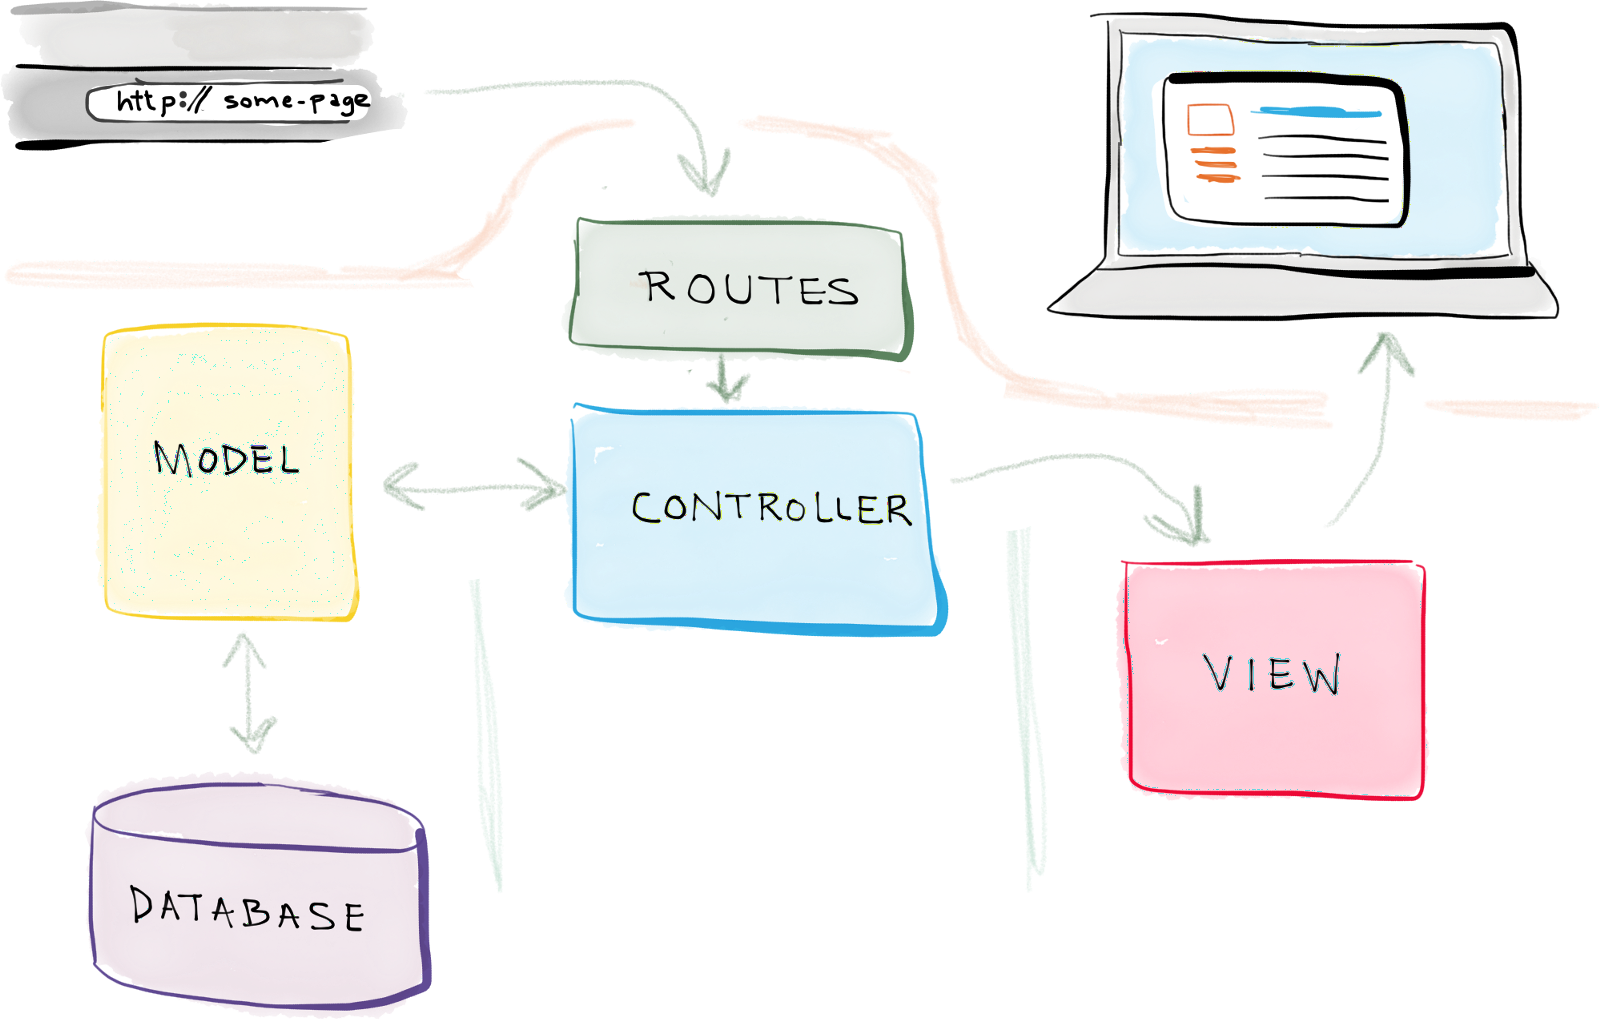
\includegraphics[width=17cm]{imgs/mvc.png}
\end{center}\vspace{-0.3cm}
\caption[The Model-View-Controller Pattern of ASP.NET Core]{The Model-View-Controller Pattern of ASP.NET Core} \label{mvc}
\end{figure}


The server-side MVC (Model-View-Controller) framework (as depicted in figure \ref{mvc} has three core layers:

\begin{enumerate}
\item \textbf{The Model}: The Model in an MVC application represents the state of the application and any business logic or operations that should be performed by it.\cite{mvc}. This is essentially a library of supporting methods which help the Controller in generating the data to pass to the View. Those methods are especially written to handle  and populate data related to the particular View and are based on libraries of more generic functions built to provide helping functions to the Model tier.

\item \textbf{The View} Views are responsible for presenting content through the user interface. In ASP.NET Core Views use the Razor view engine which is a compact, expressive and fluid template mark-up language for defining views using embedded C\# code.  Razor is predominantly used to dynamically generate web content on the server and allows to cleanly mix server code with client side content and code. \cite{mvc}. Razor view engine is also used for the opposite; embed c\# code in HTML mark-up. As a general principle, there should be minimal, if not none, logic within the views, and any logic should be related to presenting the content/model, passed from the Controller.

\item \textbf{The Controller}: This is a set of classes that manages the relationship between the View and the Model\cite{mvcBook}. It responds to user input, communicates with the Model, and ``decided'' which view to render and send back to the client side. Essentially, it controls the application logic for a particular unit and is responsible to call all the necessary methods from the Models in order to generate and pass the correct data to the View.

\end{enumerate}

\section{Design Class Diagram}
\label{design_class_diagram}


The design class diagram represents a complete overview of the classes within the system, the methods they use and the links between them. On of the main aims of designing the class diagram, is to achieve high cohesion and low coupling. The design class diagram, shown in Figure \ref{DesignClassDiagram} fully details all the internal entities of the system and maps the structure of the components of the software. As explained in subsection \ref{sub:MVC} the controller classes contain methods which are responsible for handling all entities of the system and updating specific states during their life-cycles, depending on the performed action. The notation used for this diagram is based on common industry notation for class diagrams \cite{entity_relationship_approach} \cite{object_oriented_modeling_and_design}.


\clearpage

\begin{landscape}
\begin{figure}[h]
\begin{center}
\thispagestyle{empty}
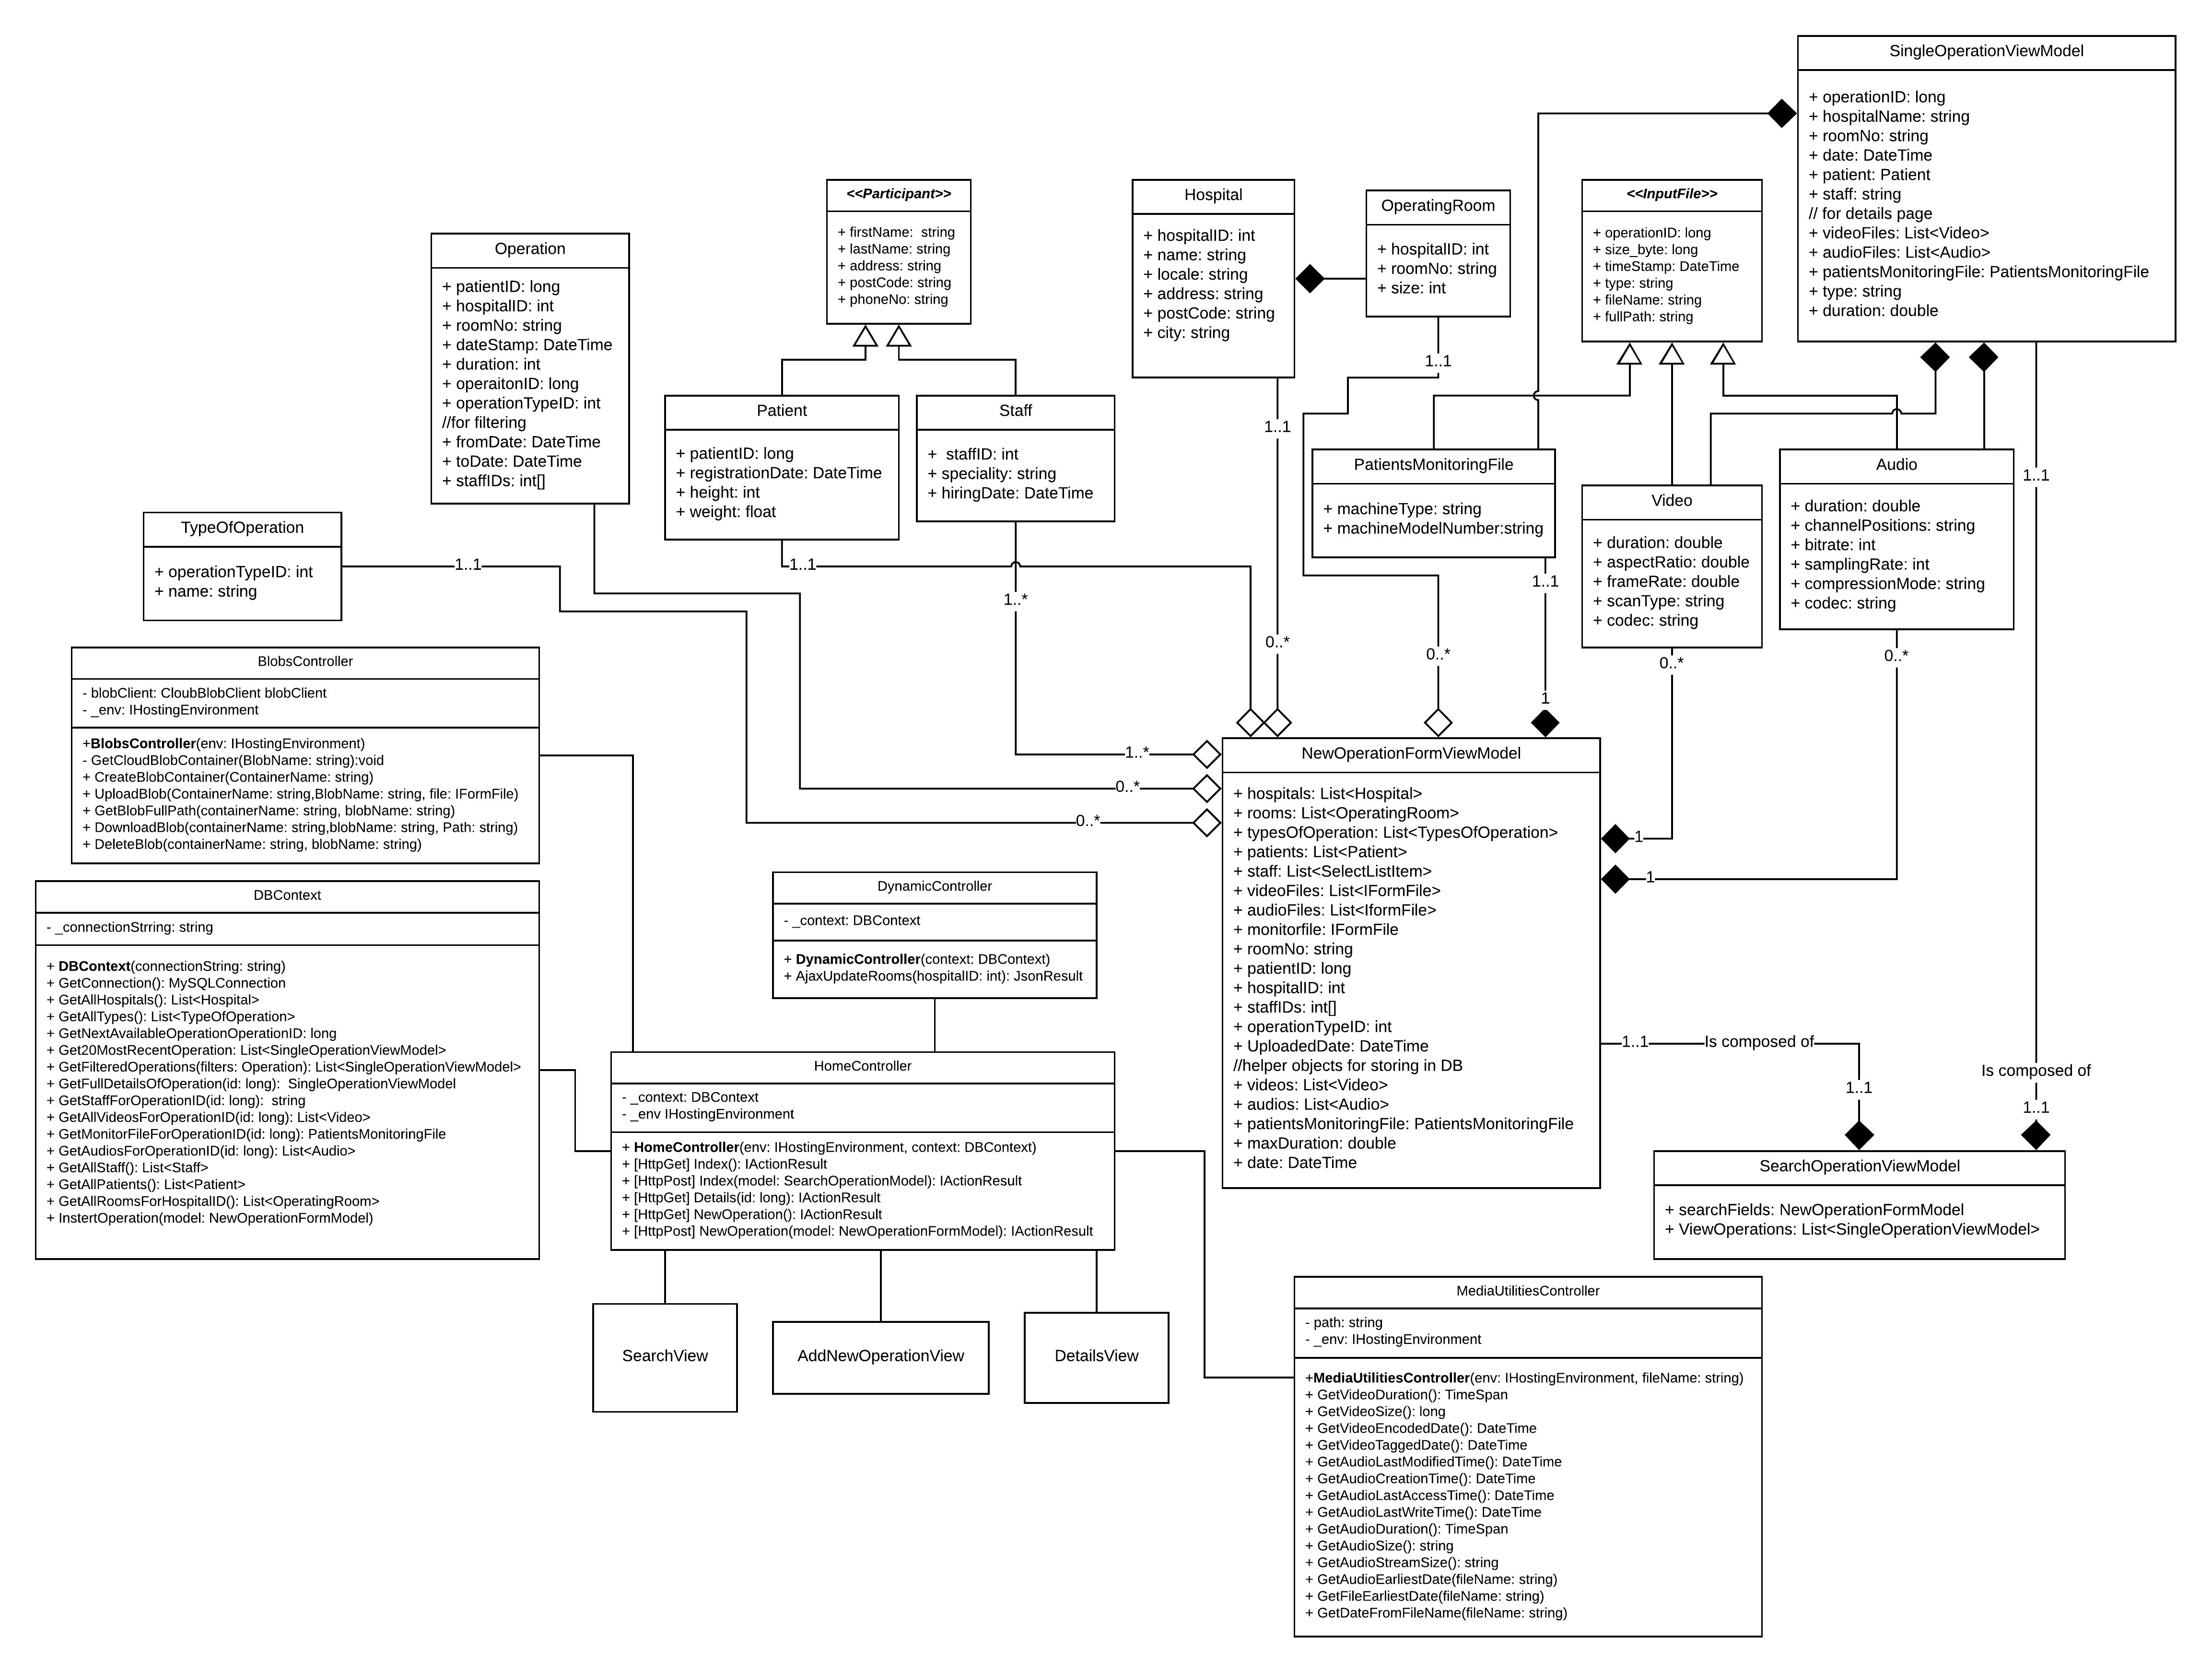
\includegraphics[width=24cm]{imgs/Design_Diagram.png}
\end{center}\vspace{-0.3cm}
\caption[Design Class Diagram]{Design class diagram.} \label{DesignClassDiagram}
\end{figure}
\end{landscape}
\newpage

 
\section{Database Design}
\label{database_design}

\subsection{Introduction}
\label{sub:intro}
A database is a data repository where the data is managed and stored according to the data structure.  It enables data sharing across an organisation, reduces data redundancy and increases data consistency. Database development doesn't have a unique way of implementing, and different data structures require different types of database. In regards to this application, the relational database was selected to represent the data structure. The main purpose of relational databases is to examine how data is related to each other. They translate the complicated data structure and data relationship into simple two-dimensional tables. In the relational model, data and relationships are represented as tables, each of which has a number of columns with a unique name.

Regarding this specific application, it was deemed that a MySQL\cite{mysql} database is the most suitable relational database management system. MySQL is an easy to use, reliable, scalable and specifically designed and optimized for Web Applications. Although it requires additional configuration when the application is deployed in the server, it is powerful enough to support the extensive complexity that the current application needs.

\subsection{Conceptual Schema}
Conceptual modeling or conceptual database design is the process of constructing a model of the information use in an enterprise that is independent of implementation details, such as the target DBMS, application programs, programming
languages, or any other physical considerations. This model is called a conceptual
data model\cite{Database_Systems}. The Conceptual Schema is shown in figure \ref{conceptual_schema}.


\begin{figure}[h]
\begin{center}
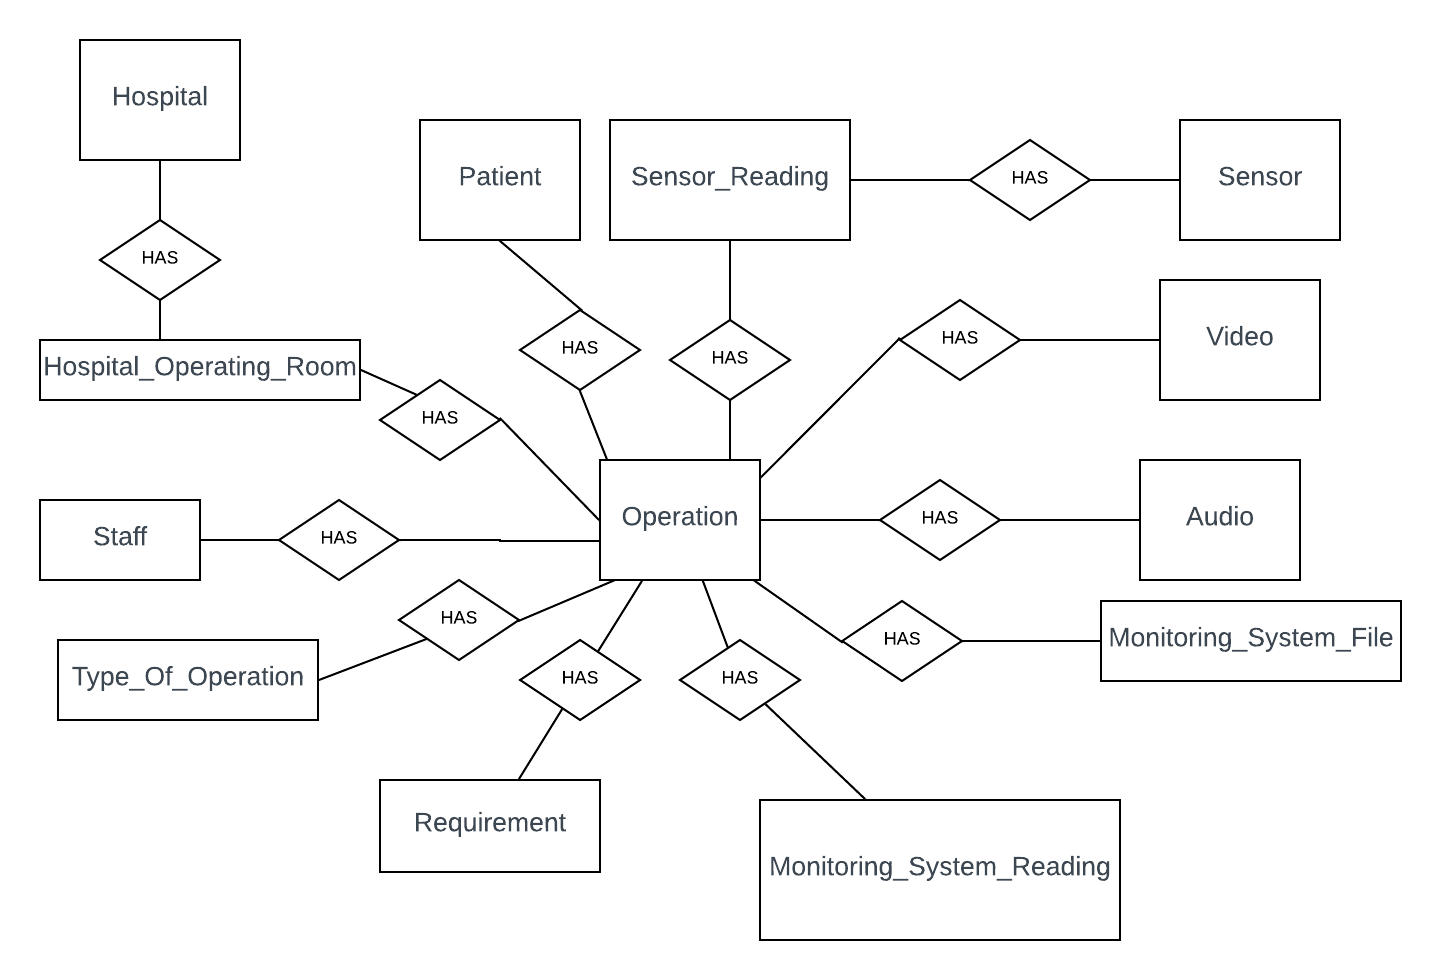
\includegraphics[width=17cm]{imgs/conceptual_schema.png}
\end{center}\vspace{-0.3cm}
\caption[Conceptual schema]{Conceptual schema} \label{conceptual_schema}
\end{figure}



\subsection{Logical Schema}

The logical database design phase maps the conceptual data model on to a logical model, which is influenced by the data model for the target database. The logical data model is a source of information for the physical design phase, providing the physical database designer with a vehicle for making trade-offs that are very important to the design of an efficient database \cite{Database_Systems}

While the conceptual model is independent of all implementation details, the logical model assumes knowledge of the underlying data model
of the target DBMS. The Entity Relationship diagram (Figure \ref{er_diagram}) is created based on the analysis of logical schema. All attributes of every entity have been labelled in the diagram.


\begin{figure}[h]
\begin{center}
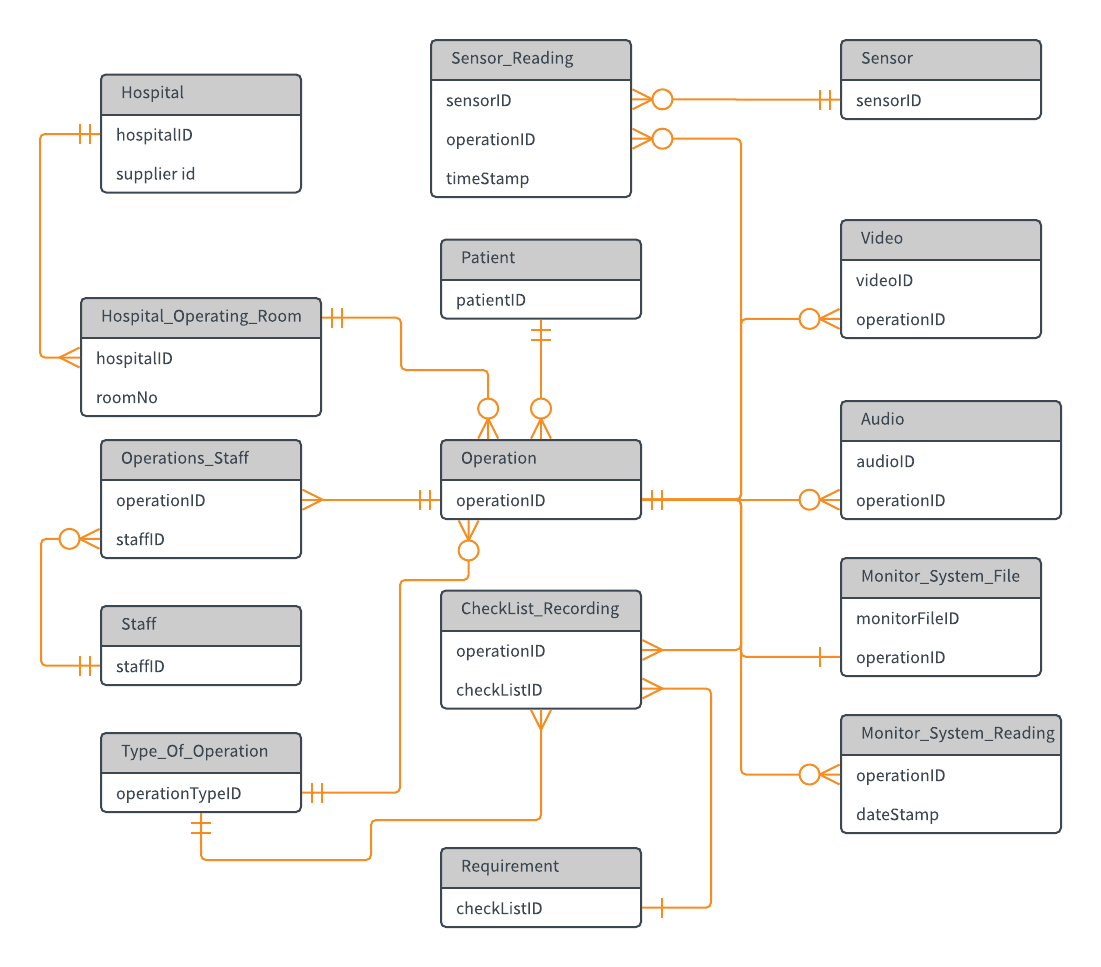
\includegraphics[width=17cm]{imgs/er_diagram.png}
\end{center}\vspace{-0.3cm}
\caption[Entity-Relationship Diagram]{Entity-Relationship Diagram} \label{er_diagram}
\end{figure}


\subsection{Physical schema}

In this final phase of the database design methodology, the logical database design (entities, attributes, relationships, and contrains) has to be translated into a physical database design that can will be implemented using the target DBMS, which in this case in a MySQL database hosted in Azure. Each attribute in the physical schema ( Figure  \ref{physical_schema} ) has constrains which prevent storing invalid data and quickens up the data validation process, requiring no additional code to rewrite the data validation interfaces. The physical database has been especially designed in order to require minimal work for new sensor adding. For example, if a new sensor is added in the future, the  schema wouldn't have to be changed and a single row in the ``Sensor'' table is the only required action. Each sensor reading is recorded to the ``Sensor\_Reading'' relation.

\begin{figure}[!ht]
\begin{center}
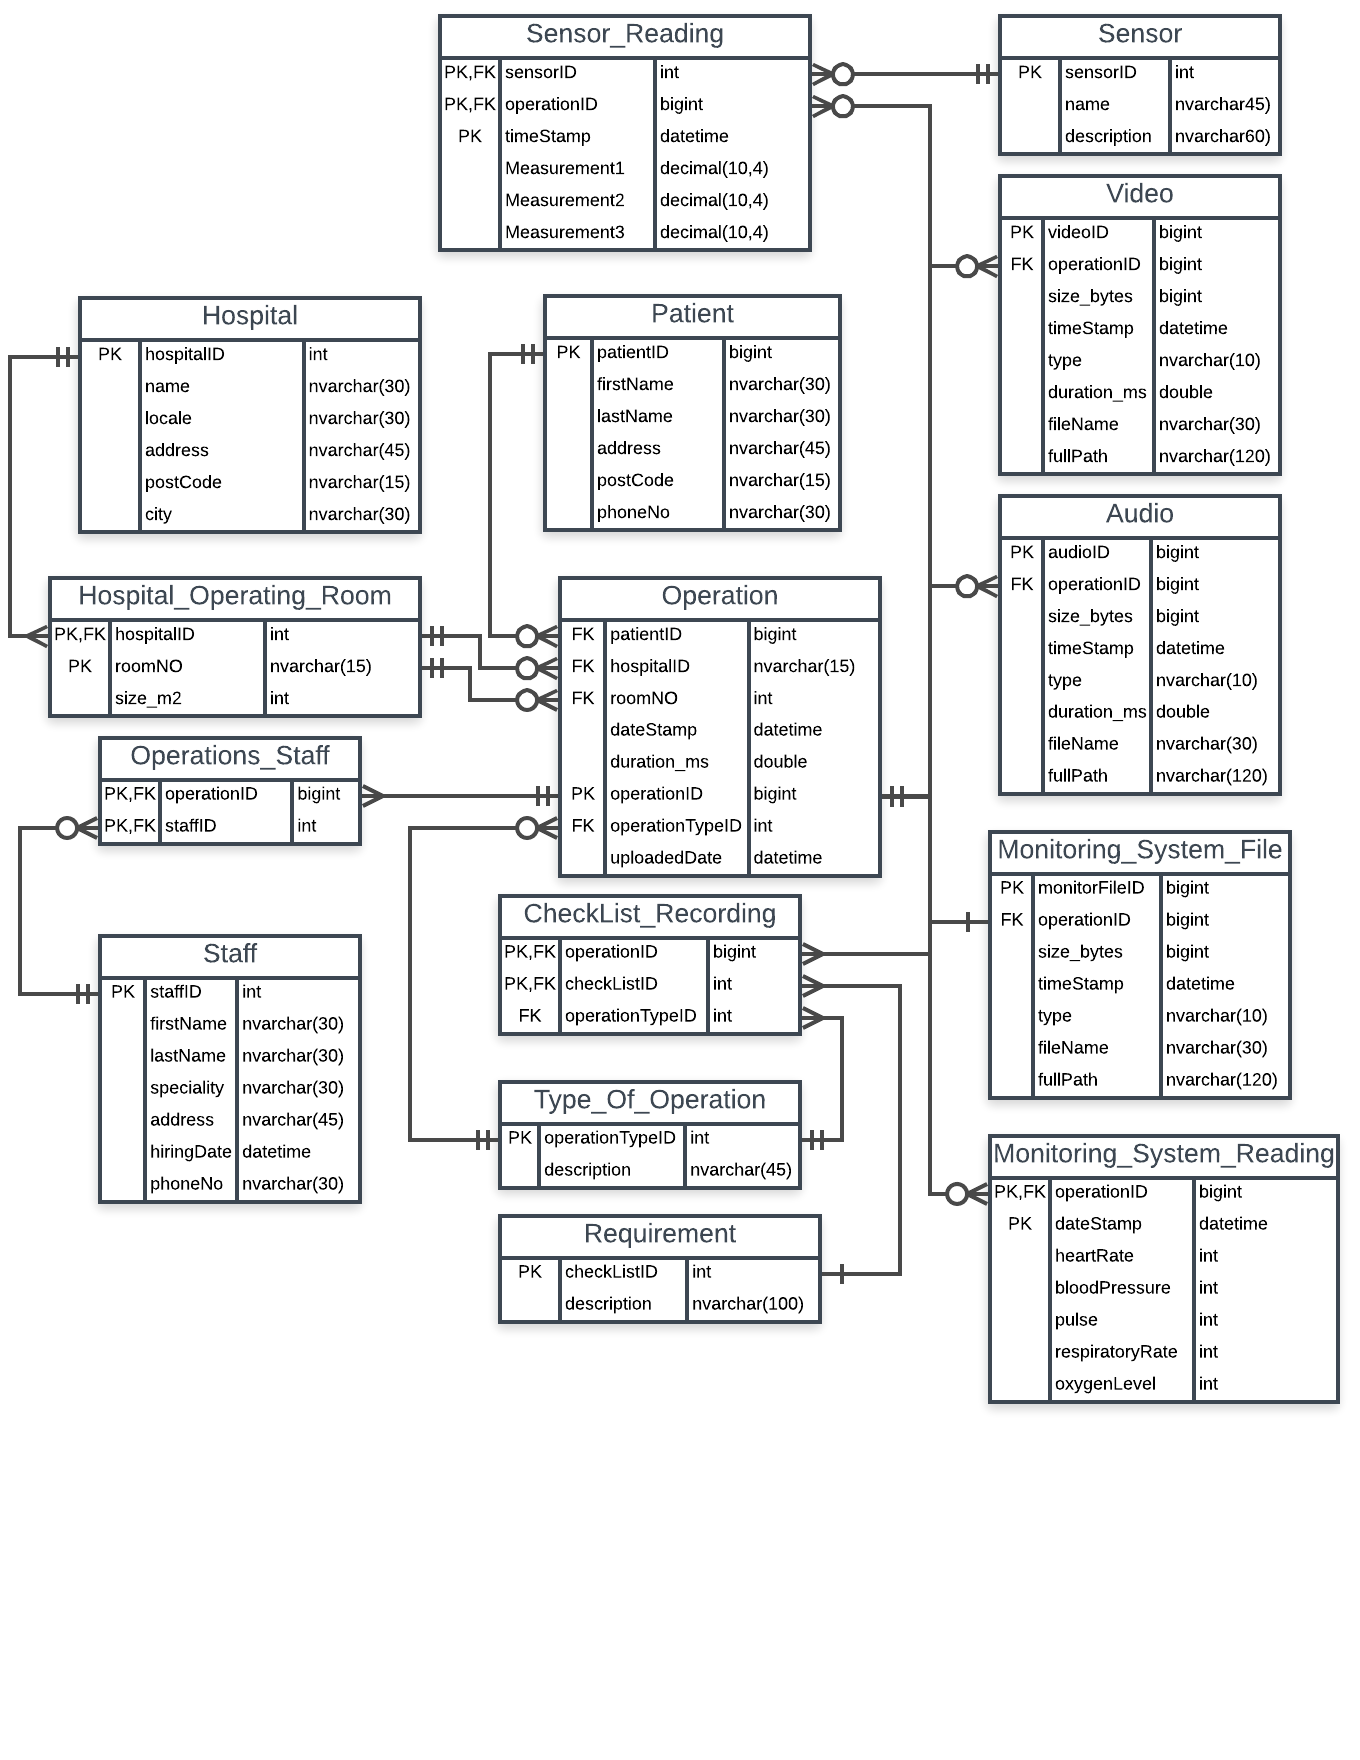
\includegraphics[width=17cm]{imgs/physical_schema.png}
\end{center}\vspace{-0.3cm}
\caption[Physical database schema]{Physical database schema} \label{physical_schema}
\end{figure}

\section{Pages Implementation}
\label{sec:pages_implementation}

Since, the front-end part of the application is fairly straight-forward, the implementation stage will be split into three subsection which are also the three main views of the application. The first part of the implementation is the page where the user can upload a new operation, the second part is where the user can make a search for a specific operation stored in the relational database and choose an operation of their choice, and the third page is where the user can see all the details that are related to the specific operation.
The application has a single Controller, which as mentioned in \ref{sub:MVC}, is an interface between the Model and the View components, processes all the logic and incoming requests, manipulates data using the Model component and interacts with the Views to render the final output. In the HomeController of the application, there are three main methods that correspond to the three main views, which will be analysed in detail in the following subsections. 


\subsection{``Register new operation'' Implementation}
\label{sub:register_new_operation_implementation}

In this subsection, the process of registering a new operation to the system is explained. The HomeController of the application has two methods with exactly the same names (``New Operation'') that correspond to the HttpGet and HttpPost request from the client side. When the user selects to load the ``Add new Operation'' View, the HttpGet method is called from the Controller. Due to the fact that this page doesn't require a already defined model of the application, a new ViewModel had to be created (``NewOperationViewModel''). 
At this stage, the controller instantiates the ViewModel, queries the database to load it and then passes it to the rendered View for display. The HttpGet method of the HomeController is shown in figure \ref{new_operation_get}.


\begin{figure}[!ht]
\begin{center}
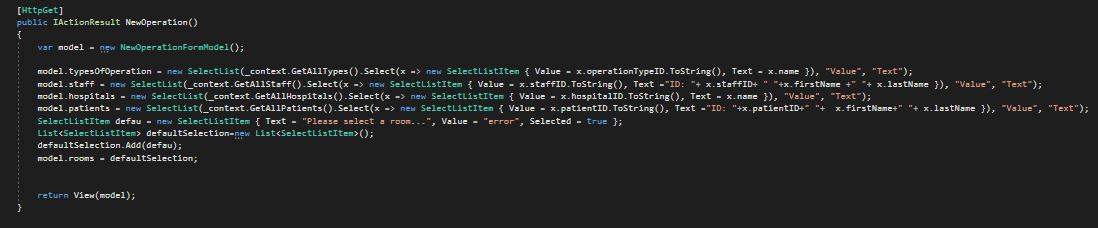
\includegraphics[width=17cm]{imgs/new_operation_get.jpg}
\end{center}\vspace{-0.3cm}
\caption[NewOperation (HttpGet Request)]{NewOperation (HttpGet Request)} \label{new_operation_get}
\end{figure}

After the model is passed to the view, all the information, in regards to the model, will be displayed. The user here, enters all the information related to the specific operation (hospital, operating room, participated staff) and uploads the input files that have been extracted from the sensors. The information entered from the user are passed to the server using the ASP.NET Core MVC Model Binding. Model binding in ASP.NET Core MVC maps data from HTTP requests to action method parameters. When MVC receives an HTTP request, it routes it to a specific action method of a controller. It determines which action method to run based on what is in the route data, then it binds values from the HTTP request to that action method's parameters \cite{modelBinding}.

Before the web application posts back to the server, JavaScript validation has to be performed to ensure that the user conforms with the application's requirements. More specifically, the user has to select a value from all the dropdown menus, and select at least one video file or one audio file or the patient's monitoring system file. The user interface that the user uploads a new operation is shown in figure \ref{new_operation_page}. It is important here to mention that the field ``Operating Room'' depends on the selection of the specific hospital and cannot be pre-populated. Therefore, a request had to be submitted to the server without posting back and so AJAX had to be used. The section where the client sends a request to the server, in order to query the database and return a JSON object is shown in figure \ref{ajax}


\begin{figure}[!ht]
\begin{center}
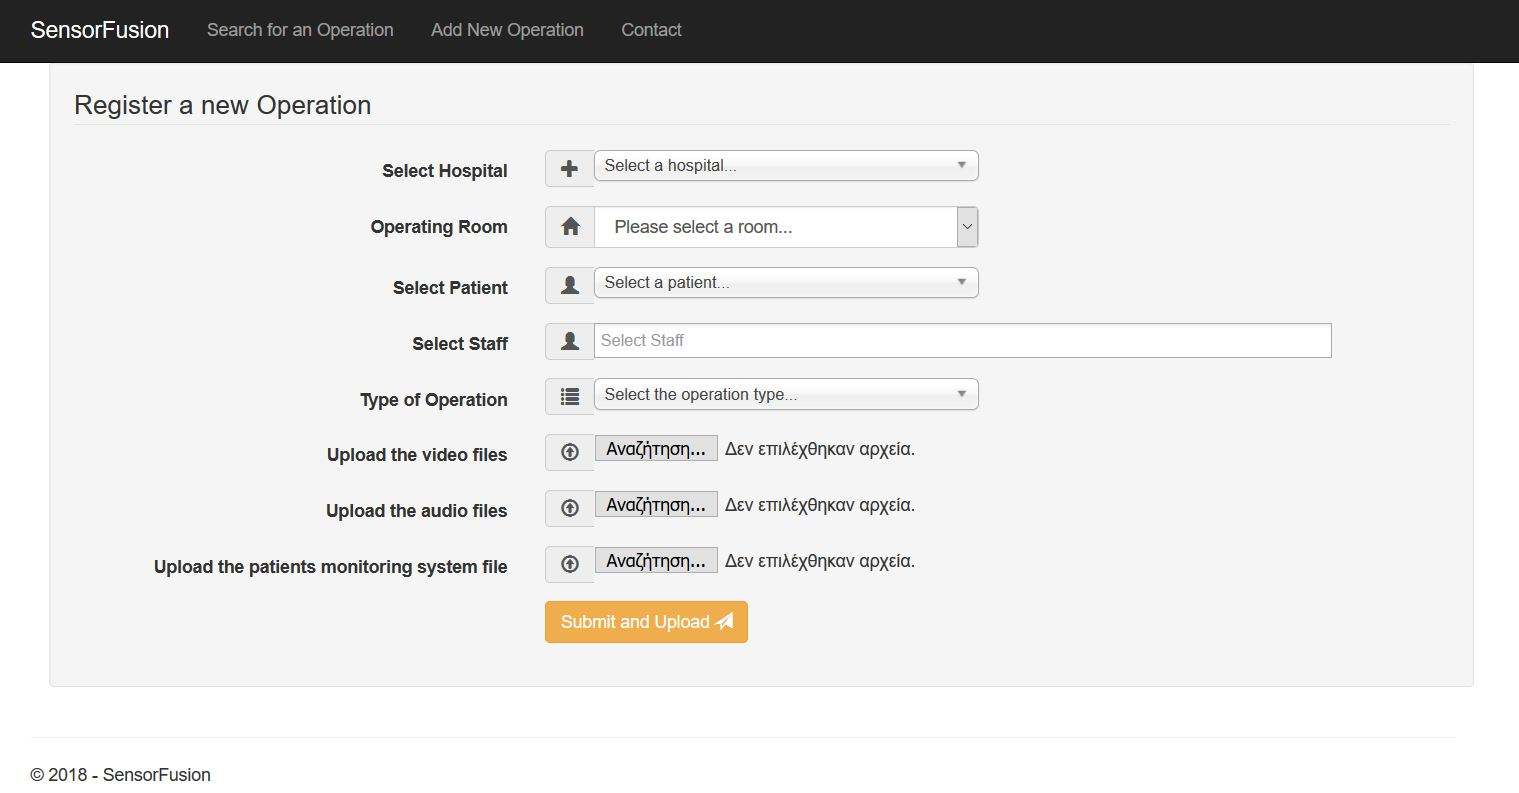
\includegraphics[width=17cm]{imgs/new_operation_page.jpg}
\end{center}\vspace{-0.3cm}
\caption[NewOperation Page]{NewOperation Page} \label{new_operation_page}
\end{figure}

\begin{figure}[!ht]
\begin{center}
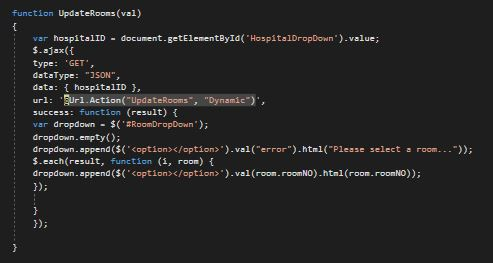
\includegraphics[width=17cm]{imgs/ajax.jpg}
\end{center}\vspace{-0.3cm}
\caption[AJAX Call]{AJAX Call} \label{ajax}
\end{figure}

When the user has entered all the required fields and selected at least one input file for uploading, a HttpPost request is submitted to the server. As previously mentioned, model binding in ASP.NET Core easily binds the data coming from the View to the model, which is then passed back to the controller for manipulation. When the user submits the form, another method with the same name is called (``NewOperation'') which is responsible for the HttpPost requests and takes as input the ViewModel (NewOperationFormViewModel).
After the server-side validation of the model has been successful, the controller must process and manipulate the incoming data, store the input files in the Azure blob storage and insert the new operation to the MySQL relational database. For the purpose of communicating with the database, an additional class has been created (DBContext). The controller, takes as input the model originated from the View, manipulates the incoming data, and passes the same model to the ``DBContext'' class for updating the database. This is a very important issue, as the application had to follow the principle of separation of concerns.
It is very critical here to mention that only the metadata extracted from the input files were stored to the MySQL database. The files themselves were only stored to a connected file storage account (Microsoft Azure Blob Storage). For this purpose, a new controller had to be created in order to store and retrieve the files from the file storage (BlobsController).

In regards to the extraction of the meta-data from the input files, additional NuGet packages and libraries (MediaInfo) had to be installed to the project. Furthermore, a dedicated class for processing, manipulating and extracting metadata from the files had to be created (``MediaUtilities''). This class enables the application to extract information from the input files that would have otherwise been almost impossible to gain. A very small sample of the obtained metadata include the exact starting date, the size of the files, codec used, encoded date, aspect ratio, frame-rate, duration of the media files and many more. The part where the application extracts the metadata from the media files is shown in figures \


\begin{figure}[!ht]
\begin{center}
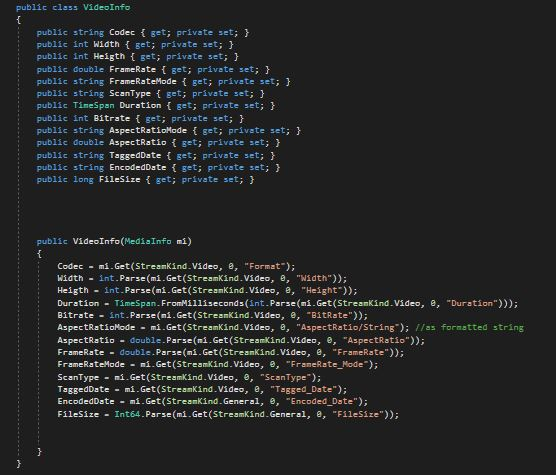
\includegraphics[width=17cm]{imgs/video_extracting.jpg}
\end{center}\vspace{-0.3cm}
\caption[Extracting meta-data from video files]{Extracting meta-data from video files} \label{video_extracting}
\end{figure}

\begin{figure}[!ht]
\begin{center}
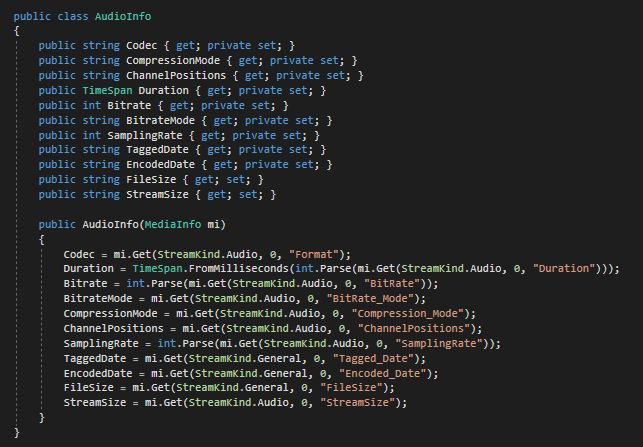
\includegraphics[width=17cm]{imgs/audio_extracting.jpg}
\end{center}\vspace{-0.3cm}
\caption[Extracting meta-data from audio files]{Extracting meta-data from audio files} \label{audio_extracting}
\end{figure}




\subsection{``Search for an operation'' Implementation}
\label{sub:search_for_an_operation_implementation}

Following the regisration of a new operation, the user can navigate to the home page, where they can search for an operation stored in the relational database. As mentioned in subsection \ref{sub:register_new_operation_implementation}, two methods with the same name were created in the HomeController, one for the HttpGet and one for the HttpPost request.


\subsection{``Operation Details'' Implementation}
\label{sub:operation_details_implentation}



\blindtext

\blindtext

\blindtext


